\chapter{Client design and development}
\label{ch:client}

\section{Page layout and styling}

\subsection{Navigation menu}

\subsection{Instructions panel}

\subsection{Main viewer}

\subsection{Button panel}

\section{Visjs variables}

\subsection{Nodes}

\subsection{Edges}

\subsection{Interaction}

\subsection{Layout}

\section{Learning process}

\begin{figure}
    \centering
    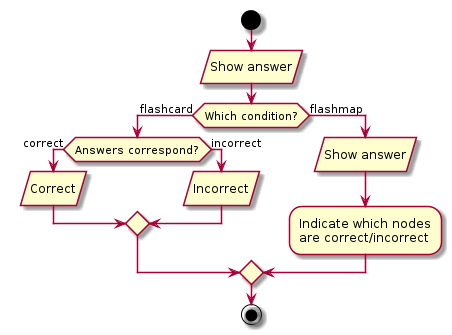
\includegraphics[width=.8\textwidth]{img/learningclient.png}
    \caption{An activity diagram displaying the prompting of an instance to the user}
    \label{fig:learningclient}
\end{figure}

\subsection{Read source}

\subsection{Flashcard prompt}

\subsection{Flashcard response}

\subsection{Flashmap prompt}

\subsection{Flashmap response}

\subsection{Finished learning}

\subsection{No more instances}

\section{Other views}

\subsection{Login screen}

\subsection{Test}

\subsection{Questionnaire}

\subsection{Debriefing}

\subsection{Main window}

\subsection{Help}

\subsection{Learning progress}
\label{sec:learningprogress}

